\documentclass[12pt]{amsart}
\usepackage{amsmath, amsthm, amssymb, graphicx, setspace, listings, float, hyperref}
\usepackage[margin=1in]{geometry}
%You will want the setspace.sty file in the same folder as your source file when you use this template

%Sets the margins
\usepackage{times,txfonts}
\usepackage{mwe}
\usepackage{caption}
\usepackage{subcaption}

%\textwidth = 6.5 in
%\textheight = 9 in
%\oddsidemargin = 0.0 in
%\evensidemargin = 0.0 in
%\topmargin = 0.0 in
%\headheight = 0.0 in
%\headsep = 0.0 in
%\parskip = 0.2in
%\parindent = 0.0in


%\begin{figure}[H]
%    \begin{center}
%        \caption{Sample Allocation Code:}
%        \lstinputlisting[language=r, basicstyle=\linespread{1}\ttfamily\small,columns=fullflexible]{r1.txt}
%        \end{center} 
%    \end{figure}

    % \begin{figure}[H]
    % \begin{center}
    % \caption{Strata Breakdown}
    % 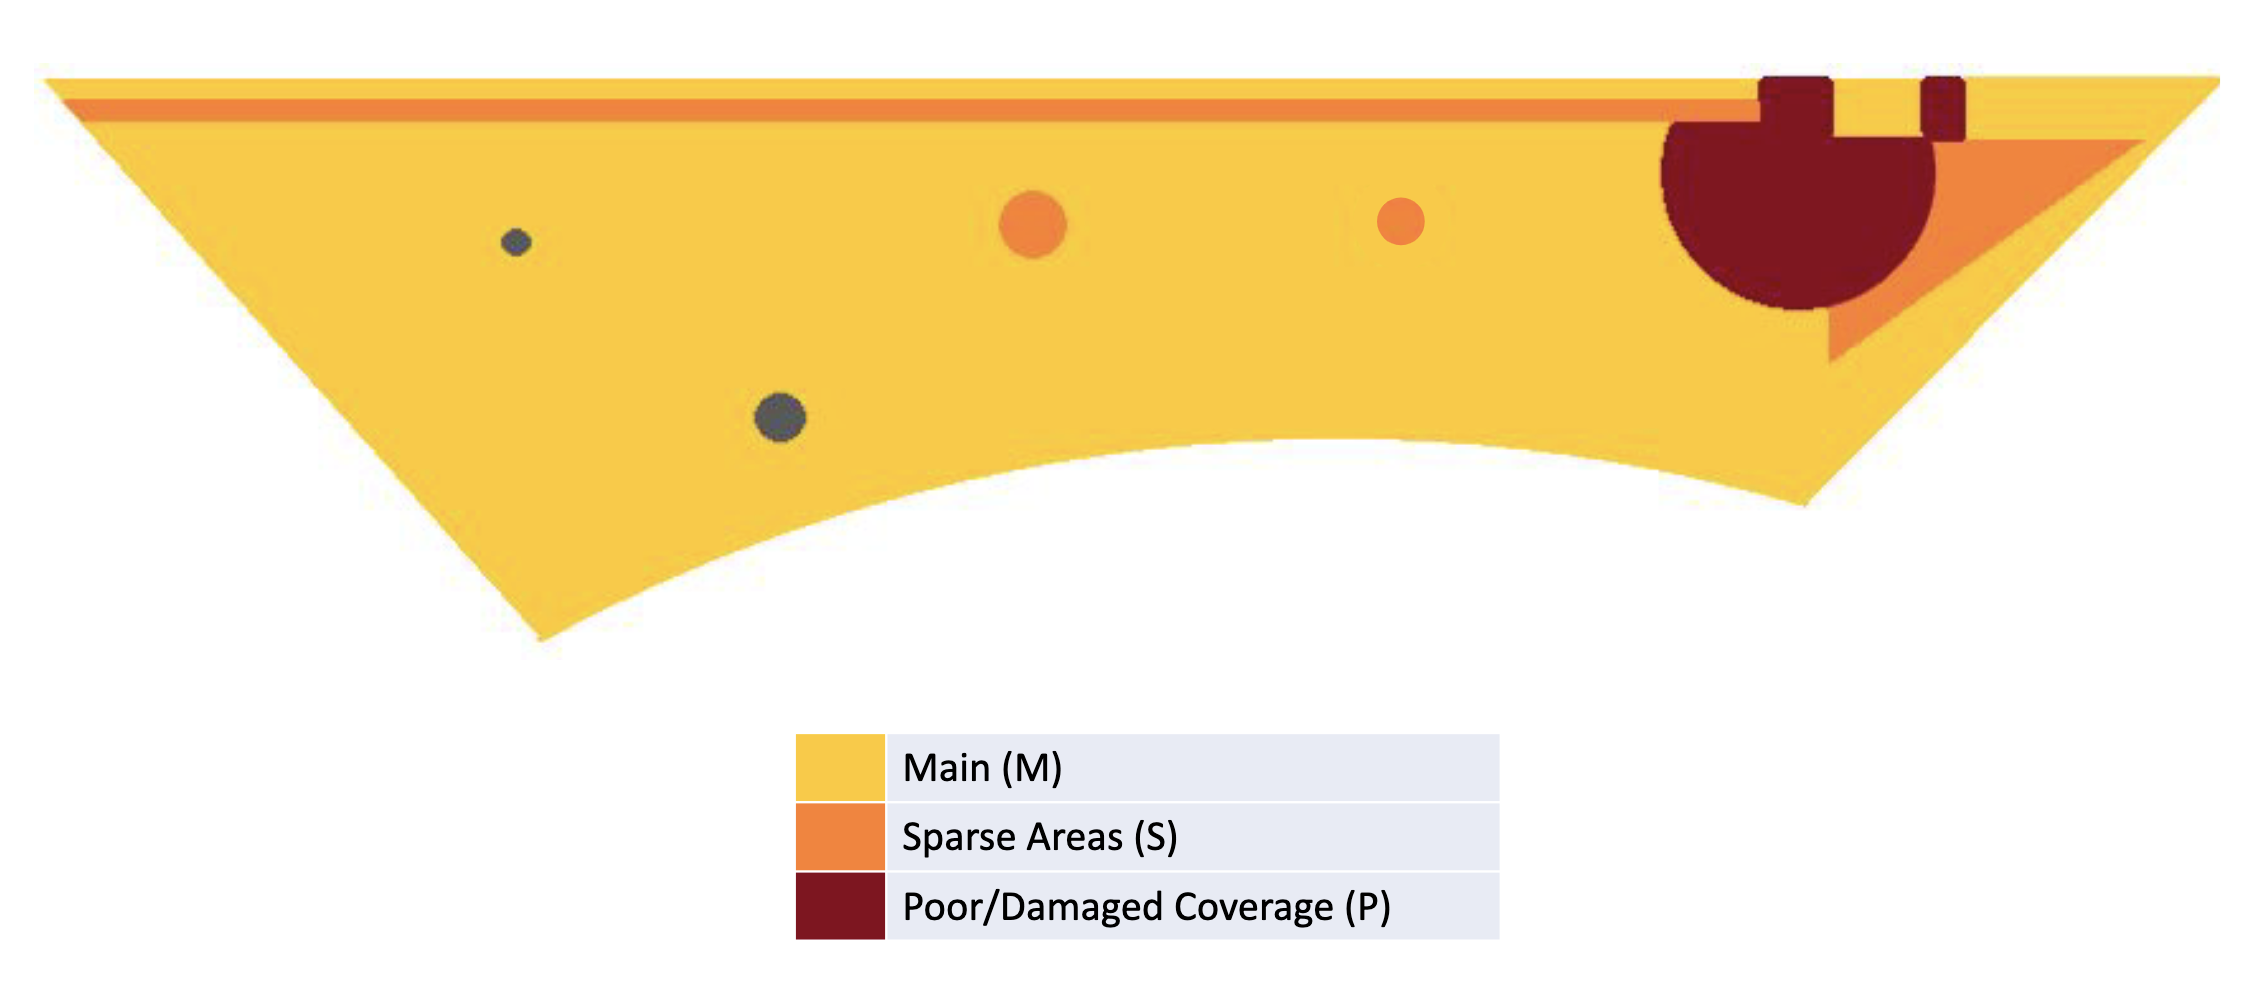
\includegraphics[width=\linewidth]{fig1.png}
    % \end{center}
    % \end{figure}


%defines a few theorem-type environments
\newtheorem{theorem}{Theorem}
\newtheorem{corollary}[theorem]{Corollary}
\newtheorem{definition}{Definition}

\title{Estimating Proportion of Birch Trees in Plot South of Reichardt}
\author{Stefano Fochesatto, Bria Hiebert-Crape, Thomas House}
\date{\today} % Uncomment and insert a date to specify a date

%%% BEGIN DOCUMENT
\begin{document}

\begin{abstract}
    Proportion data was collected from the plot directly south of the Reichardt building at UAF during the Fall 2021 semester. 
    The plot was organized into 173 north to south transects to facilitate an arms-length sample width. The entire population of trees 
    in each transect was then sampled, thus performing a one-stage cluster sample. Our group decided on taking 6 samples, two for each sampler. 
    The proportions estimate was computed using the usual one-stage cluster sample proportion estimator. 
\end{abstract}

\doublespacing %%INCLUDE THIS TO DOUBLESPACE!


\maketitle
%\renewcommand{\baselinestretch}{1.2}

\section*{Area Study}%Change what's in brackets to change the section title.
\subsection*{Initial Survey and Area Analysis}
With satellite imagery we found that the full length of the plot as measured on the northernmost side came out to be 865 feet. An initial survey found the proportion of birch trees in the 
plot to be very low and relatively clustered together. The plot contained mainly three species of trees: spruce, aspen, and birch. \\
The transects were plotted north to south to span all elevations, despite being more difficult to sample. We decided to make each 
transect about arms-length to make it easier to sample every tree in the transect. With the width of each transect and the length of the northernmost 
side we can compute the total number of transects(clusters) through division. 


\section{Sample Allocation and Methods}
Our group decided to sample only 6 samples and divide them evenly among each group member. Since we are using single stage cluster sampling 
we can always sample more clusters to improve our estimate. With the total number of transects computed (N) and the total number of transect samples (n)
decided, we computed a simple random sample of the transects in r to decide which transects to sample. 
\begin{figure}[H]
    \begin{center}
        \caption{Sample Allocation Code:}
        \lstinputlisting[language=r, basicstyle=\linespread{1}\ttfamily\small,columns=fullflexible]{SRSClusters.r}
        \end{center} 
    \end{figure}
The midpoint of our sampled transects was computed as the length across the northernmost side of the plot starting from the west. Doing so we could create the following map to illustrate the location of our samples, 
 \begin{figure}[H]
 \begin{center}
 \caption{Transect Breakdown}
 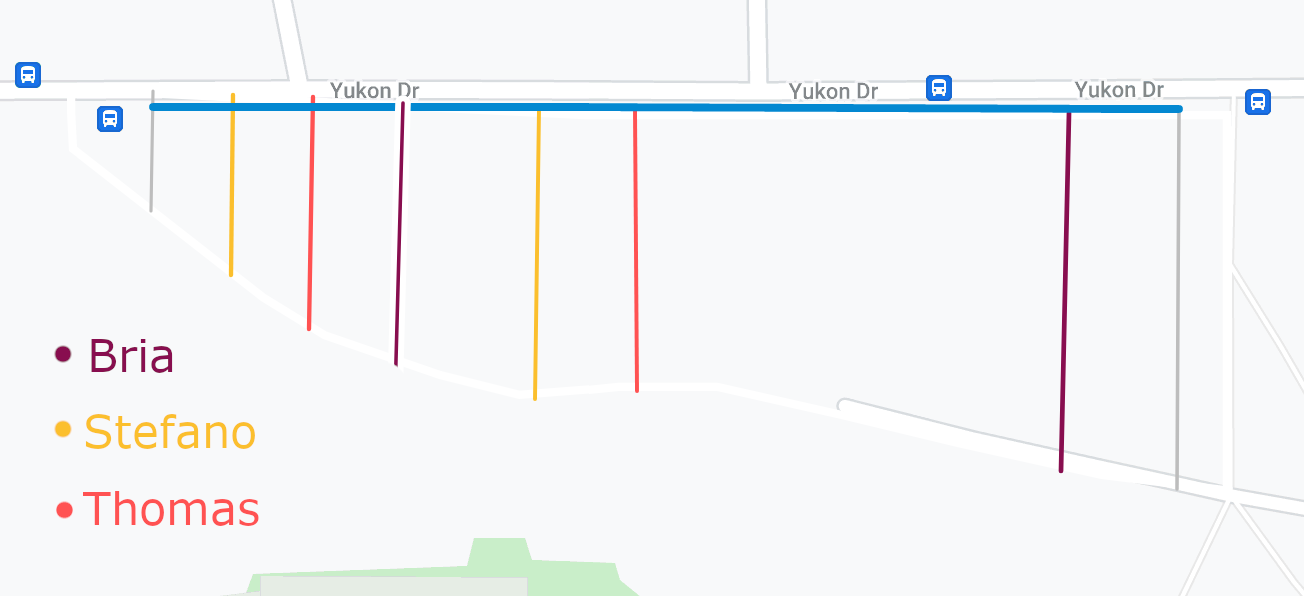
\includegraphics[width=\linewidth]{AreaImageEdited.png}
 \end{center}
 \end{figure}
Sampling occurred by walking down the middle of each transect and considering each tree within an arms-length. The circumference of each tree was measured using a cardboard tool in order to 
enure that each tree in our sample had a circumference greater than 4 inches. 


\begin{figure}[H]
    \centering
    \begin{subfigure}[b]{0.45\textwidth}
        \centering
        \includegraphics[width=\textwidth]{SampledTree.png}
        \caption{Example of a Sampled Tree}

    \end{subfigure}
    \hfill
    \begin{subfigure}[b]{0.45\textwidth}
        \centering
        \includegraphics[width=\textwidth]{NotSampledTree.png}
        \caption{Example of a Not Sampled Tree}

    \end{subfigure}
       \caption{Circumference Determination}
\end{figure}

\section{Results}
From our six transects the following data was collected. 
\begin{figure}
    \caption{Data Table}
\begin{center}
    \begin{tabular}{||c c c||} 
     \hline
     Sampler & \# of Birch & \# of Aspen and Spruce  \\ [0.5ex] 
     \hline\hline
     Stefano & 0 & 10 \\ 
     \hline
      & 3 & 16  \\
     \hline
     Bria & 2 & 15 \\
     \hline
      & 0 & 7  \\
     \hline
     Thomas & 0 & 14  \\ 
     \hline
      & 1 & 5  \\ [1ex] 
     \hline
    \end{tabular}
    \end{center}
\end{figure}
Recall the formula for computing the proportion estimator with a single stage cluster sample, 
\begin{equation*}
    \hat{p} = \dfrac{\sum_{i = 1}^{n} \tau_i }{\sum_{i = 1}^{n} M_i }.
\end{equation*}
Now recall the formula for computing the variance, 
\begin{equation*}
    \hat{V}(\hat{p}) = \left(\dfrac{N - n}{N}\right)\left(\dfrac{N}{M}\right)^2\left(\dfrac{MSE}{n}\right),
\end{equation*}
\begin{equation*}
    MSE = \dfrac{\sum_{i = 1}^{n}(\tau_i - \hat{p}M_i)^2}{n-1}.
\end{equation*}
Recall that since we don't know M(the number of trees in the plot) we need to estimate the following term, 
\begin{equation*}
    \dfrac{N}{M} \approx \frac{n}{\sum M_i}.
\end{equation*}
Computing the the estimator, variance and 95 percent confidence interval in r, we get the following. 
\begin{figure}[H]
    \begin{center}
        \caption{Estimator Computation Code:}
        \lstinputlisting[language=r, basicstyle=\linespread{1}\ttfamily\small,columns=fullflexible]{rAnalysis.r}
        \end{center} 
    \end{figure}



\section{Conclusion}
To summarize, our estimator gave us that the proportion of birch trees in the plot is  0.08219178 with 
a 95 percent confidence interval between (0.1482569, 0.0161267). From my experience sampling an exploring the plot 
these results seem reasonable, and thankfully if we desired a tighter confidence interval we could easily go back out to the 
plot and sample more clusters. Designing the clusters so that they were an arms-length wide in combination with the fact that 
we used a simple random sample for our clusters, made our sampling scheme very versatile. As a sampler I would say that collecting 
data for this projects was very straightforward, and easy while also delivering decent results for relatively small effort. 


\end{document}
















